\chapter{Contexte g\'en\'eral}
\section{Introduction}
Ce chapitre abordera comme sujet la situation du contexte g\'en\'eral du projet, sur un niveau organisationnel en pr\'esentant l'organisme d'accueil, et sur un niveau contextuel qui refl\`ete la motivation et les objectifs du projet ainsi que la m\'ethodologie de travail durant son d\'eroulement.
\section{Pr\'esentation de l'organisme d'accueil}

\subsection{Office ch\'erifien des phosphates}

L'Office Ch\'erifien des Phosphates \`a sa cr\'eation, le Groupe OCP, depuis 1975, a \'evolu\'e sur le plan juridique, pour devenir en 2008 une soci\'et\'e anonyme d\'enomm\'ee ${\triangleleft}$ OCP S.A ${\triangleright}$.

D'une activit\'e d'extraction et de traitement de la roche \`a ses d\'ebuts, OCP s'est positionn\'e au fil du temps sur tous les maillons de la chaine de valeur, de la production d'engrais \`a celle d'acide phosphorique, en passant par les produits d\'eriv\'es. L'OCP trouve, depuis sa cr\'eation, les ressources de sa croissance continue et de son leadership dans sa strat\'egie industrielle. Celle-ci est rythm\'ee par une mont\'ee en puissance r\'egulid\`ere de l'outil de production, par une politique ambitieuse de partenariats durables et servie par une politique financid\`ere efficace.

Ces partenariats touchent aussi bien des accords de livraison \`a moyen et \`a long terme que la construction d'unit\'es de production sous forme de jointventures, bas\'ees au Maroc et \`a l'\'etranger. Aujourd'hui, OCP compte douze filiales et joint-ventures ainsi que quatre bureaux de repr\'esentations dans le monde.

Depuis sa cr\'eation, OCP est pass\'e de quelques centaines de personnes \`a prd\`es de 23 000 collaborateurs et 46 milliards de DH de chiffre d'affaires en 2013.

Afin de mener \`a bien la transformation digitale du Groupe OCP, l'entit\'e ${\triangleleft}$ Digital Office ${\triangleright}$ s'organise autour des principes manag\'eriaux suivants :

\begin{itemize}
\item Flexibilit\'e et agilit\'e dans l'allocation des ressources humaines dans une logique d'efficacit\'e et ce, \`a travers une structuration en pools permettant l'agilit\'e dans le staffing, la r\'eduction des niveaux hi\'erarchiques, ainsi que le renforcement de la collaboration et de l'autonomie.
\item Ouverture forte vers les m\'etiers, dans une logique de d\'emarche centr\'ees utilisateur, par la mise en place d'interfaces m\'etiers pour capturer et challenger leurs besoins dans un objectif de cr\'eation de valeur .
\item Stimulation et accompagnement \`a l'innovation par le d\'eploiement de capacit\'es d'innovation technologique et d'acculturation digitale .
\item Synergies entre les entit\'es Digitales et celles du Systd\`eme d'Information pour concilier les besoins d'agilit\'e avec les enjeux de stabilit\'e, de s\'ecurisation et de p\'erennisation du socle SI, assurant par l\`a-même le succd\`es de la transformation.
\end{itemize}

En application de ces principes, l'entit\'e ${\triangleleft}$  Digital Office ${\triangleright}$ est structur\'ee comme suit :

\begin{itemize}
\item Une ${\triangleleft}$ {\color{orange}{Digital Factory}} ${\triangleright}$ avec des antennes sur les diff\'erents sites du Groupe, en charge de livrer les initiatives digitales de la feuille de route, dans des cycles d'it\'eration courts, \`a travers des m\'ethodes de fonctionnement agile autour d'\'equipes cross-fonctionnelles .
\item Une entit\'e ${\triangleleft}$ {\color{orange}{Syst\`emes d'Information}} ${\triangleright}$, en charge d'assurer la r\'ealisation des projets SI, le bon fonctionnement des infrastructures SI et t\'el\'ecoms du Groupe, ainsi sue l'assistance et le support aux utilisateurs du Groupe, dans le respect des exigences de qualit\'e et des meilleurs standards en la mati\`ere .
\item Une entit\'e ${\triangleleft}$ {\color{orange}{Data Management}} ${\triangleright}$ en charge d'\'elaborer une strat\'egie et un mod\`ele de gouvernance de la Data, de d\'efinir l'architecture Data sein du Groupe, et de mettre en \oe uvre les initiatives data y aff\'erentes .
\item Une entit\'e ${\triangleleft}$ {\color{orange}{Data Planning \& PMO}} ${\triangleright}$, en charge de la construction et de la mise \`a jour de la roadmap digitale du Groupe et du suivi de son ex\'ecution .
\item Une Entit\'e ${\triangleleft}$ {\color{orange}{Business Architecture}} ${\triangleright}$, en charge de conseiller et challenger les m\'etiers sur les solutions digitales pertinentes pour adresser leurs besoins, les consolider et suivre leur mise en \oe uvre .
\item Un pool ${\triangleleft}$ {\color{orange}{Digital Innovation \& Change Officers}} ${\triangleright}$, en charge d'identifier et mener des projets d'innovation en mati\`ere de Digital (veille technologique, prototypage, Open Innovation ...), ainsi que de la promotion d'une culture digitale et de nouveaux modes de travail au sein du Groupe .
\end{itemize}

\begin{figure}[!htb]
	\center{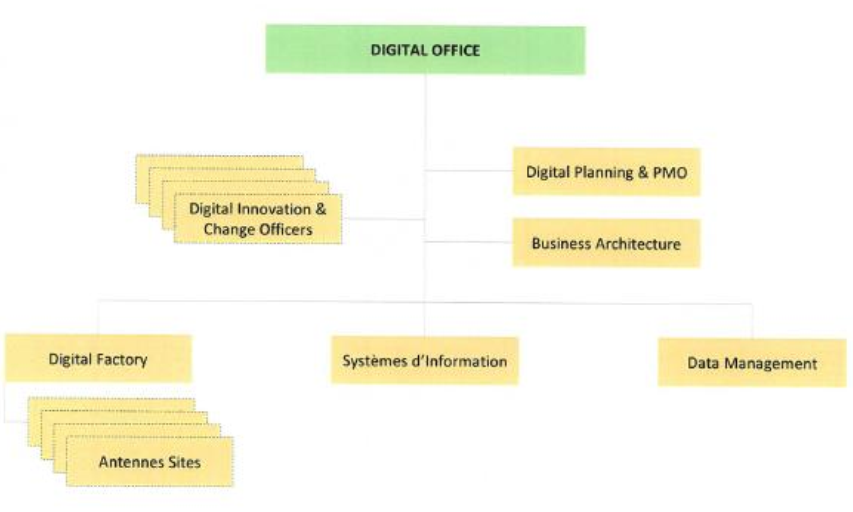
\includegraphics[width=0.8\textwidth]{Figures/digitalOffice.PNG}}
	\caption{\label{fig:my-label} Structure de la Digital Office de l'OCP}
\end{figure}

\subsection{L'importance de la digitalisation}

Le digital est un incubateur de nouveaux modes de fonctionnement \`a l'\'echelle du Groupe. Il favorise l'intrapreneuriat, la prise d'initiative et r\'einvente la mani\`ere d'interagir avec l'\'ecosyst\`eme du Groupe. Le digital repr\'esente aussi un gisement consid\'erable en termes d'innovations et de d\'eveloppement industriel et favorise l'\'emergence de nouveaux talents au sein du Groupe OCP et de son \'ecosyst\`eme.
Le challenge de cette transformation digitale r\'eside dans la diffusion d'une culture digitale aupr\`es de l'ensemble des collaborateurs et la conception de solutions innovantes pour enrichir et supporter les diff\'erents m\'etiers d'OCP.

\subsubsection{Objectifs}

\begin{itemize}
\item[\textbf{Renforcer l'efficacit\'e op\'erationnelle}]\ :anticiper les changements et agir en temps r\'eel \`a travers la promotion de l'Advanced Analytics , augmenter les capacit\'es de production, r\'eduire les co\^ots, et construire une Supply Chain agile, int\'egr\'ee et adapt\'ee \`a un march\'e dynamique.

\item[\textbf{Se connecter aux agriculteurs et aux clients}]\ :\^etre plus proches de leurs besoins, enjeux et probl\'ematiques et leur proposer des exp\'eriences ( fully digitized ).

\item[\textbf{D\'evelopper de nouveaux produits et services}]\ :augmenter la flexibilit\'e pour am\'eliorer l'existant et cr\'eer de nouvelles offres.

\item[\textbf{Explorer de nouvelles voies de croissance}]\ :introduire des m\'ethodologies de gestion de projets plus agiles, rapides et fluides, \`a travers des cycles de conception et d'innovation plus courts.
\end{itemize}

\subsection{La Digital Factory de l'OCP}

La vision digitale du Groupe OCP consiste \`a devenir un organisme de digitalisation phare de l'industrie dans la r\'egion, ainsi que et favoriser l'innovation et les moyens num\'eriques de travailler dans l'ensemble de l'organisation.

\begin{figure}[!htb]
	\center{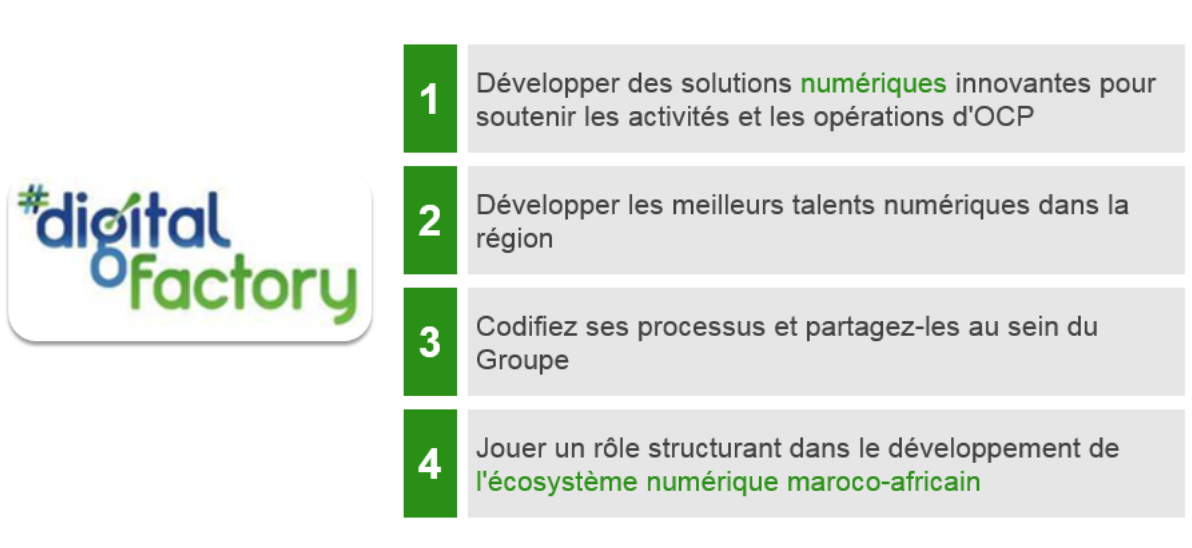
\includegraphics[width=\textwidth]{Figures/digitalFactory.PNG}}
	\caption{\label{fig:my-label} les buts majeurs de la Digital Factory de l'OCP}
\end{figure}

Le Groupe OCP a construit sa nouvelle entit\'e ${\triangleleft}$ Digital Factory ${\triangleright}$ qui sera \`a la pointe de l'innovation et de la transformation num\'erique de toute l'organisation et au-del\`a.

La Digital Factory rassemble les comp\'etences, les processus, la culture, et les points d'entr\'ees afin de mener la transformation digital et de livrer des produits digitaux. Elle vise \`a :

\begin{itemize}
\item Construire la capacit\'e interne \`a poss\'eder la d\'efinition et la livraison de produits num\'eriques
\begin{itemize}
\item R\'eduire le ${\triangleleft}$ time to market ${\triangleright}$
\item Augmenter la qualit\'e de la livraison
\item Mettre l'accent sur l'impact et les r\'esultats
\end{itemize}
\item Mettre \`a l'\'echelle une culture transformative
\begin{itemize}
\item Fournir un plan pour l'avenir du travail qui dynamise l'entreprise et encourage les employ\'es
\item Cr\'eer un vortex pour l'innovation et la cr\'eativit\'e qui attire les meilleurs talents de l'int\'erieur et de l'ext\'erieur de l'organisation
\end{itemize}
\end{itemize}

\section{Pr\'esentation g\'en\'erale du projet}
La Digital Factory de l'\gls{OCP} a entam\'e une nouvelle phase de digitalisation avanc\'ee relative au processus de gestion des anomalies. Ceci permettra aux employ\'ees d'une part d'avoir en temps r\'eel, l'ensemble des informations relatives \`a chaque \'etape du processus. Depuis l'alert du probl\`eme jusqu'\`a leur r\'esolution et d'autre part, offrira de la transparence pour \^etre plus performant et \'economiser en temps et ressources.

L'objectif g\'en\'erale du projet est de r\'ealiser une application web \& mobile qui sera utiliser par trois types des employ\'es :
\begin{itemize}
\item \textbf{Prospecteur} : dont le r\^ole est d'assurer la qualit\'e / quantit\'e de phosphates en auditant les sites d'extraction.
\item \textbf{Exploitant} : dont le r\^ole est d'assurer la continuit\'e de l'exploitation (machines, pilotes ...).
\item \textbf{Administrateur} : dont le r\^ole est de g\'erer l'application. 
\end{itemize}
\subsection{Pr\'esentation du projet de fin d'\'etudes}
L'extraction du phosphate dans les mines de Khouribga suivent les cinq \'etapes suivantes :

\begin{figure}[!htb]
	\center{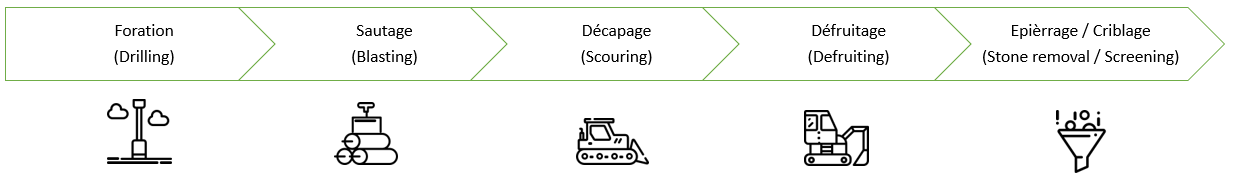
\includegraphics[width=\textwidth]{Figures/5steps.PNG}}
	\caption{\label{fig:my-label} Les cinq \'etapes d'extraction du phosphate}
\end{figure}

Les prospecteurs fournissent des informations g\'eologiques aux responsables des op\'erations (Exploitant) avant le d\'ebut du premier forage, puis suivent l'\'evolution jusqu'\`a l'extraction du phosphate.

Apr\`es le d\'ecapage, la premi\`ere couche du phosphate est visible et le prospecteur peut pr\'elever un \'echantillon pour d\'eterminer la qualit\'e du phosphate (HT: Haute Teneur, BT: Basse Teneur ...).
Disons que le premier \'echantillon pr\'elev\'e \'etait HT, mais apr\`es avoir analys\'e et stock\'e le phosphate, nous avons fait un autre test et la qualit\'e \'etait BT.

Pour \'eviter cette situation, le travail de Prospector consiste \`a assurer la qualit\'e / quantit\'e du phosphate extrait avant de le stocker et \`a \'eliminer toute anomalie en v\'erifiant et en v\'erifiant toutes les 5 \'etapes de l'extraction du phosphate.

\begin{figure}[!htb]
	\center{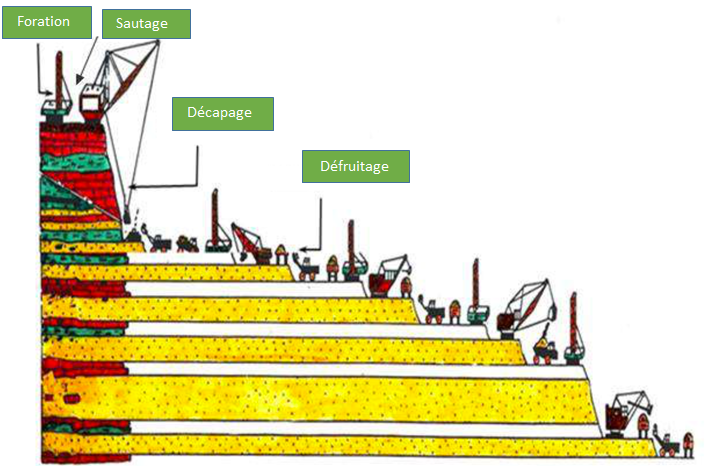
\includegraphics[width=0.8\textwidth]{Figures/levels_shema.png}}
	\caption{\label{fig:my-label} Cha\^ine cin\'etique d'extraction de phosphate}
\end{figure}

Les prospecteurs n'ont aucun support num\'erique lors de leurs inspections quotidiennes. Ils donnent toujours des instructions \`a Machine Conductors et \`a Operations Manager (Exploitant) verbalement, sans autre syst\`eme de suivi que les appels t\'el\'ephoniques ou les conversations directes.

{\color{red}{Comment pouvons-nous aider les prospecteurs \`a relever et \`a garder trace des anomalies au cours de leur inspection quotidienne pour \'eviter les souillures au phosphate?}}

\subsection{Exigences du projet}
Apr\`es une examination au terrain, les utilisateurs de notre application ont des exigences n\'ecessaires qu'on doit les respecter :
\subsubsection{Besoins des prospecteurs}
\begin{itemize}
\item S'assurer que la qualit\'e du phosphate est conforme.
\item S'assurer que le phosphate a \'et\'e completement exploit\'e
\item Communiquer facilement avec les exploitants de la mine
\item Mesurer et suivre les anomalies remont\'e lors de sa tourn\'ee.
\end{itemize}
\subsubsection{Besoins des exploitants}
\begin{itemize}
\item Terminer son shift sans incident.
\item Diriger son \'equipe avec plus d'efficacit\'e
\item Lib\'erer le chantier le plus rapidement possible
\item Veillez au respect des consignes des Prospecteurs
\item S'assurer que toutes les machines sont fonctionnelles
\end{itemize}

\subsection{Objectifs du Projet}

Les exigences initiales indiquent que la solution sera une application mobile aidant les prospecteurs et les exploitants \`a effectuer leur inspection quotidienne.

\begin{itemize}
\item R\'ep\'etition des consignes et anomalies
\item Aucun moyen de suivi des anomalies remont\'ees 
\item Disponibilit\'e de l'Exploitant sur chantier
\item Moyens de communications limit\'es entre le prospecteur et l'exploitant
\item Le t\'el\'ephone ne capte pas tou jours dans les mines 
\end{itemize}

\`A l'aide d'une s\'erie d'invites, nous pouvons r\'esoudre le probl\`eme initial et d\'efinir une feuille de route claire et coh\'erente qui nous aidera \`a d\'evelopper un MVP.

En les aidant \`a se sentir en s\'ecurit\'e et \`a \^etre productifs.

\section{Conduite du projet}
\subsection{Organisation du projet}
Apr\`es avoir pass\'e une p\'eriode de documentation et d'int\'egration au sein de la Digital Factory de l'OCP, j'ai int\'egr\'e une \'equipe qui se constitue de 6 personnes tout en respectant la structure d'une \'equipe dans le cadre Scrum.
La figure suivante illustre l'architecture de notre \'equipe :

\begin{figure}[!htb]
	\center{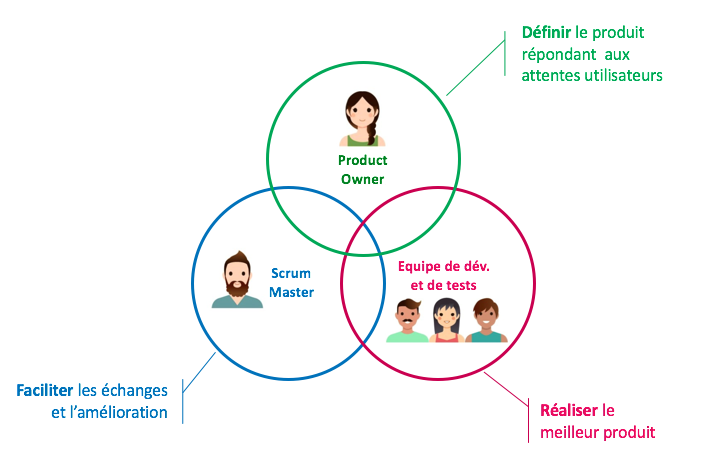
\includegraphics[width=0.8\textwidth]{Figures/scrumEquipe.png}}
	\caption{\label{fig:my-label} \'Equipe de projet}
\end{figure}

\begin{itemize}
\item Product Owner (PO),
\item 1 \'equipe de d\'eveloppement constitu\'ee de 3 d\'eveloppeurs,
\item 1 Scrum Master (SM).
\end{itemize}

Notre \'equipe Scrum est auto-organis\'ees et pluridisciplinaire. C'est \`a dire nous choisissons la meilleure fa${\c{c}}$on d'accomplir notre travail, au lieu d'\^etre dirig\'ees par des personnes externes \`a l'\'equipe.

\section{M\'ethodologie de travail}
\subsection{M\'ethodologie Scrum}
Afin de d\'erouler le projet dans des conditions standards qui s'inspirent des m\'ethodologies de travail les plus efficaces et dans le cadre de mon \'equipe de travail nous avons choisi la m\'ethodologie Scrum pour la gestion du projet.

Le choix de cette m\'ethodologie est d\^u \`a plusieurs raisons. Dans un premier temps cette m\'ethodologie favorise la productivit\'e au sein d'une \'equipe de d\'eveloppement en travaillant sur des objectifs prioritaires et \`a court terme et en suivant un d\'eveloppement it\'eratif et incr\'emental avec une planification \'evolutive bas\'ee sur la division de l'ensemble des t\^aches selon des unit\'es qu'on appelle sprint. Aussi le choix de cette m\'ethodologie tiens en compte la tendance du contexte de d\'eveloppement dans le monde qui r\'eside dans l'adaptation de l'esprit agile durant la r\'ealisation des projets, un esprit ou Scrum est l'une de ses m\'ethodologies piliers.

Le choix de Scrum comme m\'ethodologie pr\'esente plusieurs avantages li\'es \`a la productivit\'e ainsi que l'organisation du travail en se basant sur des rôles d\'efinis, ce qui n'existe pas dans les m\'ethodologies traditionnelles, qui repr\'esentent plusieurs inconv\'enients, ceux de la rigidit\'e ainsi que la g\'en\'eration massive de la documentation et la difficult\'e d'introduction des changements. Ceci justifie le choix de Scrum comme m\'ethodologie de d\'eveloppement qu'on r\'esume selon une vision d'ensemble dans la figure suivante :
\begin{figure}[!htb]
	\center{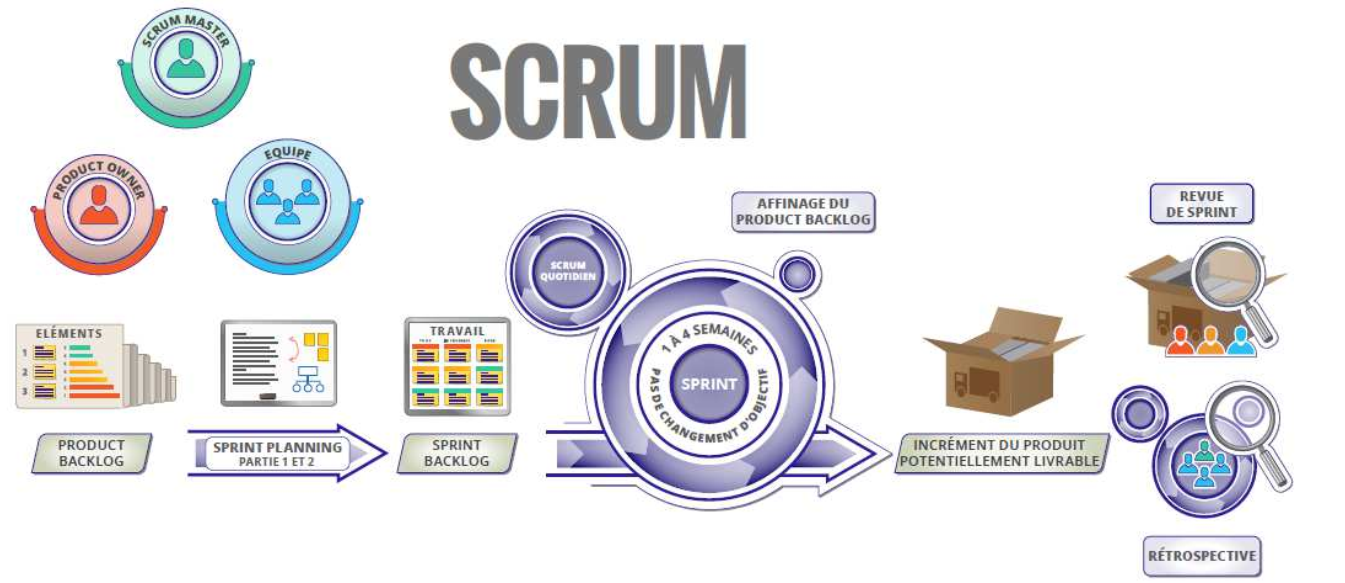
\includegraphics[width=\textwidth]{Figures/scrum.PNG}}
	\caption{\label{fig:my-label} M\'ethode SCRUM}
\end{figure}

Comme le montre la figure la r\'epartition des taches se fais selon des roles bien pr\'ecis. Dans notre cas, l'\'equipe se constitue de 8 personnes ayant les profiles suivant :
\begin{itemize}
\item[\textbf{Le PO(Product Owner)}]\ : c'est un expert m\'etier qui d\'efinit dans un premier temps les sp\'ecifications fonctionnelles. Aussi, il \'etablit la priorit\'e des fonctionnalit\'es \`a d\'evelopper ou corriger et valide les fonctionnalit\'e d\'evelopp\'ees. Bref, le PO joue le r\^ole du client.
\item[\textbf{Le Scrum Master}]\ : c'est expert Agile qui s'assure que les principes et les valeurs de Scrum sont respect\'es. Il assure la communication au sein de l'\'equipe ainsi que la recherche d'am\'elioration de la productivit\'e et du savoir-faire de notre \'equipe.
\item[\textbf{UX Designer}]\ : il fait le design de chaque user story selon l'exp\'erience d'utilisateur (user experience). L'UX design a plus un rôle de (conception de produit) qu'un rôle de conception graphique.
\item[\textbf{L'\'equipe de d\'eveloppement}]\ : constitu\'ee de 6 personnes qui s'occupent du d\'eveloppement des user stories ainsi que la r\'ealisation des tests unitaires et des tests d'int\'egration.
\end{itemize}


\subsection{Outils de suivi}

\subsubsection{JIRA Atlassian}

Le framework agile Scrum repose entre autres sur le principe de (transparence). Certaines informations doivent donc \^etre accessibles par tous, comme la t\^ache en cours de chacun, son \'etat d'avancement, et l'objectif actuel de l'\'equipe. D'o\`u l'importance que ces informations soient visibles en permanence.

C'est le tableau Scrum qui va jouer ce r\^ole. Il permet d'organiser le backlog, les t\^aches du sprint en cours et leur \'etat d'avancement. Les tableaux Scrum peuvent \^etre aussi simples qu'un tableau blanc et des posts-its, ou peuvent rev\^etir un format plus \'elabor\'e avec des logiciels sp\'ecialis\'es disposant de graphiques et de fonctionnalit\'es de gestion des t\^aches plus avanc\'ees.

Pour notre tableau Scrum,nous utilisons JIRA Atlasian. Notre tableau est divis\'e en 5 listes qui correspondent au flux de travail des t\^aches:

\begin{itemize}
\item \textbf{\`A Faire}: quand je planifie mon sprint, je d\'eplace les t\^aches du backlog vers cette liste.
\item \textbf{En Cours} : contient les t\^aches en cours de d\'eveloppement et de r\'ealisation.
\item \textbf{Termin\'e} : la t\^ache est compl\`ete dans la phase du d\'eveloppement mais en attente de la validation fonctionnelle par le PO
\item \textbf{Approuv\'e} : une fois la t\^ache est approuv\'ee fonctionnellement par le PO on peut la placer dans la colonne APPROUV\'E.
\item \textbf{Bloqued}: j'utilise cette liste lorsque la finalisation d'une t\^ache d\'epend d'un facteur externe (par exemple, je dois r\'ealiser un achat et obtenir l'aval de mon PO), en sp\'ecifiant les raisons du blocage dans un commentaire.
\end{itemize}

\begin{figure}[H]
	\center{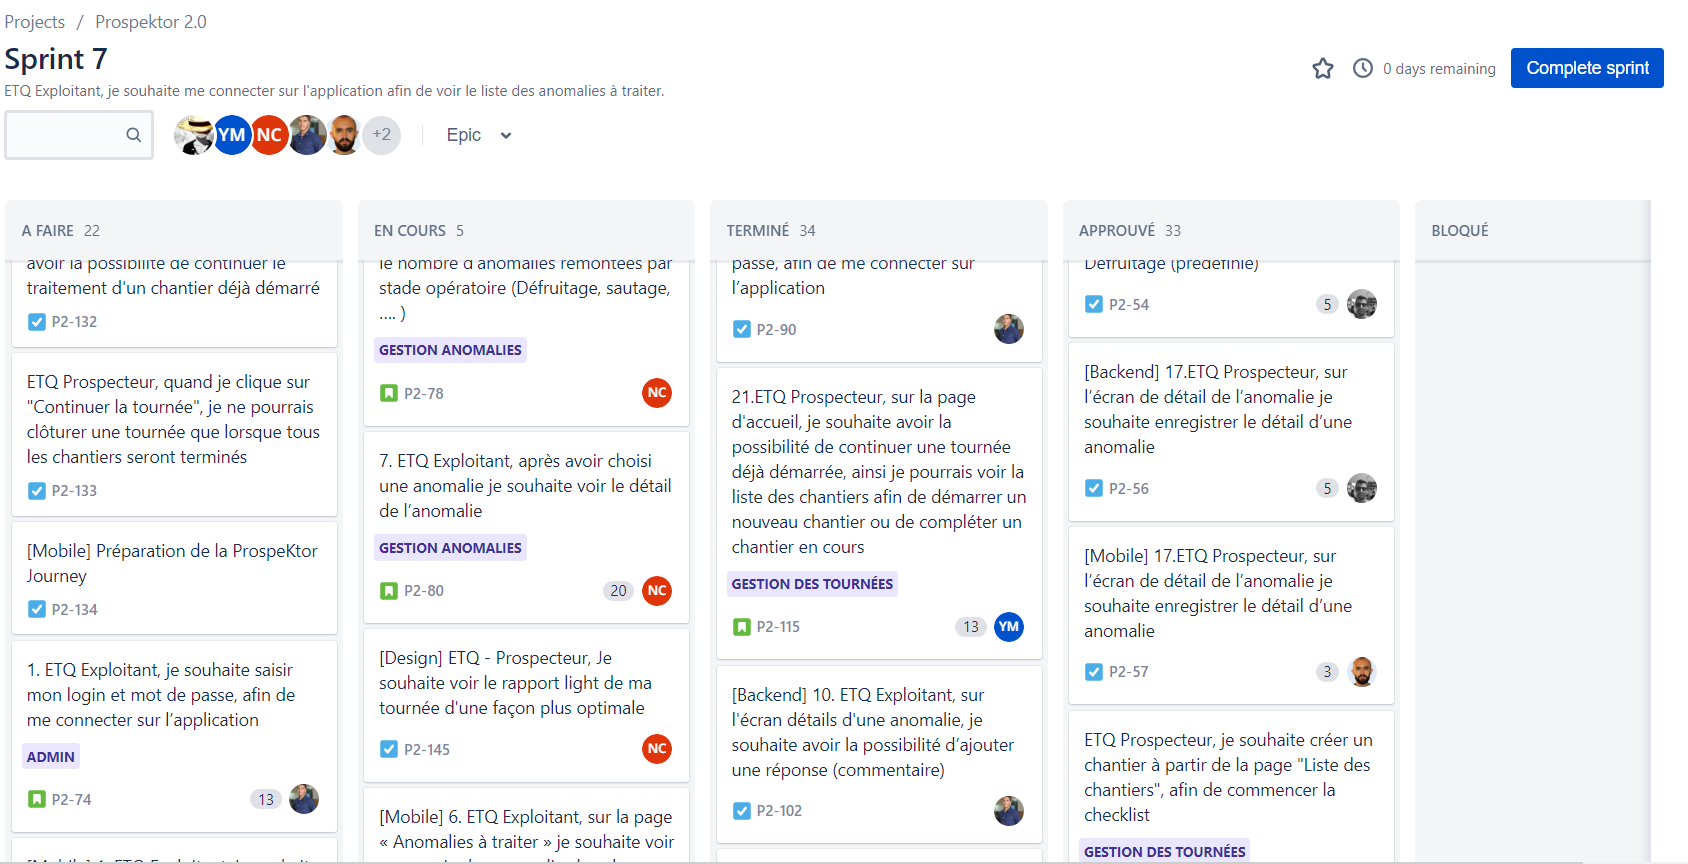
\includegraphics[width=\textwidth]{Figures/jira.png}}
	\caption{\label{fig:my-label} Capture de l'outil JIRA}
\end{figure}

\subsubsection{Slack}

Slack est une plateforme de communication collaborative sur ordinateur et smartphone. Chaque entreprise peut cr\'eer un groupe priv\'e sur Slack, et y inviter tout ou partie de ses employ\'es, qui peuvent ainsi discuter entre eux.

Avec les conversations instantan\'ees class\'ees par (cha\^ines), la communication se fluidifie, il est possible d'interagir en temps r\'eel, tout en s'adressant uniquement aux personnes concern\'ees, au contraire de l'e-mail.

L'autre atout de l'application : toutes les interconnexions qu'elle permet avec d'autres logiciels. L'outil Slack est pratique pour recevoir une notification d\`a chaque modification dans un document Drive.

\begin{figure}[H]
	\center{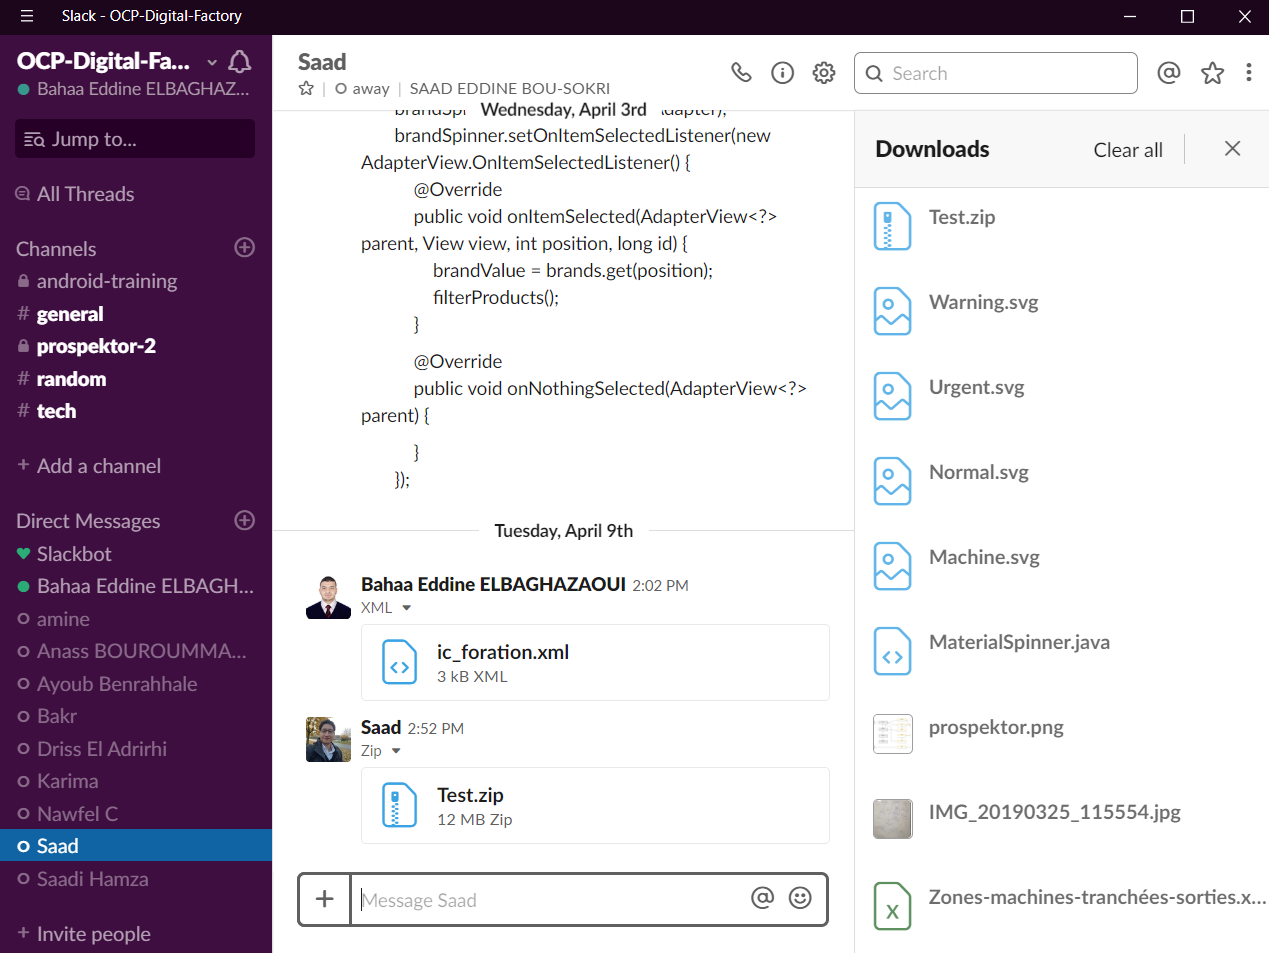
\includegraphics[width=0.5\textwidth]{Figures/slack.png}}
	\caption{\label{fig:my-label} Capture de l'outil Slack}
\end{figure}

\section{Conclusion}

Dans ce chapitre nous avons pr\'esent\'e l'ensemble des \'el\'ements qui permettent la situation de notre Projet de Fin d'\'etudes dans son contexte organisationnel ainsi que la d\'emarche de gestion du projet qui organise son d\'eroulement et les outils utilis\'es. Par la suite dans le chapitre suivant on va mettre l'accent sur l'\'etape de l'analyse et sp\'ecification des besoins qui permettra la collection des diff\'erents besoins afin de concevoir une solution qui r\'epondra aux exigences exprim\'ees